\documentclass[compress, aspectratio=169]{beamer}

%presentation layout

\mode<presentation>
{
  \usetheme{Berlin}
  % \usecolortheme{dove}
  \setbeamercolor{structure}{bg=white,fg=black}
  \setbeamercolor{normal text}{bg=white,fg=black}
  \setbeamercolor{titlepage}{bg=white,fg=black}
  \setbeamercolor{titlelike}{bg=white,fg=black}
  \setbeamercolor{palette primary}{bg=white}
  \setbeamercolor{palette secondary}{bg=gray, fg=white}
  \setbeamercolor{palette tertiary}{bg=gray, fg=white}
  \setbeamercolor{palette quarternary}{bg=white}
  \setbeamercovered{transparent}
  \useinnertheme{rectangles}
  %\usefonttheme{serif}
}

\setbeamertemplate{navigation symbols}{}

%loading packages
\usepackage[ngerman]{babel}
\usepackage[T1]{fontenc}
\usepackage[utf8]{inputenc}
\usepackage{graphicx}
\usepackage{amsmath}
\usepackage{framed}
\usepackage{caption}
\usepackage{subcaption}
\usepackage{multicol}

% vorgeplaenkel
\title[StAPf-Bericht]{StAPF-Bericht}

\author{Ständiger Ausschuss aller Physikfachschaften}

\institute[Zusammenkunft aller Physikfachschaften]

\date{20. Mai 2020}

\subject{Bericht des StAPF}

\begin{document}

\begin{frame}[plain]{}
  \titlepage
\end{frame}

\section{Mitglieder}

\begin{frame}{Gewählte Mitglieder}
  \begin{minipage}{.28\textwidth}
    \begin{figure}
      \begin{minipage}[c]{.57\textwidth}
        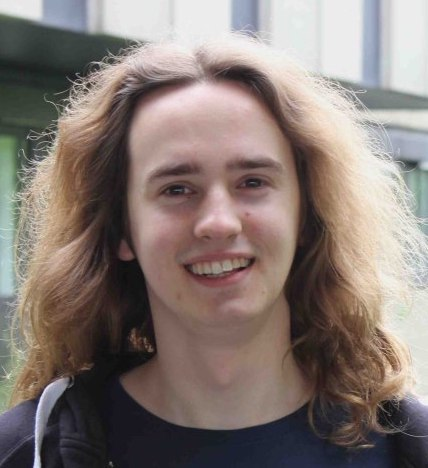
\includegraphics[height=0.3\textheight]{andy.jpg}
      \end{minipage} \hfill
      \begin{minipage}[c]{.4\textwidth}
        \caption*{Andreas Drotloff\\Uni Würzburg}
      \end{minipage}
    \end{figure}
  \end{minipage}
\hfill
  \begin{minipage}{.28\textwidth}
    \begin{figure}
      \begin{minipage}[c]{.5\textwidth}
        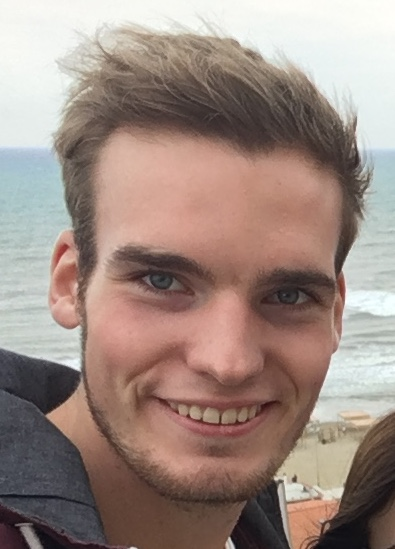
\includegraphics[height=0.35\textheight]{chris.jpeg}
      \end{minipage} \hfill
      \begin{minipage}[c]{.47\textwidth}
        \caption*{Christoph Blattgerste\\Uni Heidelberg}
      \end{minipage}
    \end{figure}
  \end{minipage}
  \hfill
  \begin{minipage}{.28\textwidth}
    \begin{figure}
      \begin{minipage}[r]{.57\textwidth}
        
\includegraphics[height=0.3\textheight]{leon.jpg}
      \end{minipage} \hfill
      \begin{minipage}[c]{.4\textwidth}
        \caption*{Leon Nutzinger \\FU Berlin}
      \end{minipage}
    \end{figure}
  \end{minipage}

  \vspace{1cm}
  \hspace{0.1\textwidth}
   \begin{minipage}{.28\textwidth}
    \begin{figure}
      \begin{minipage}[c]{.57\textwidth}
        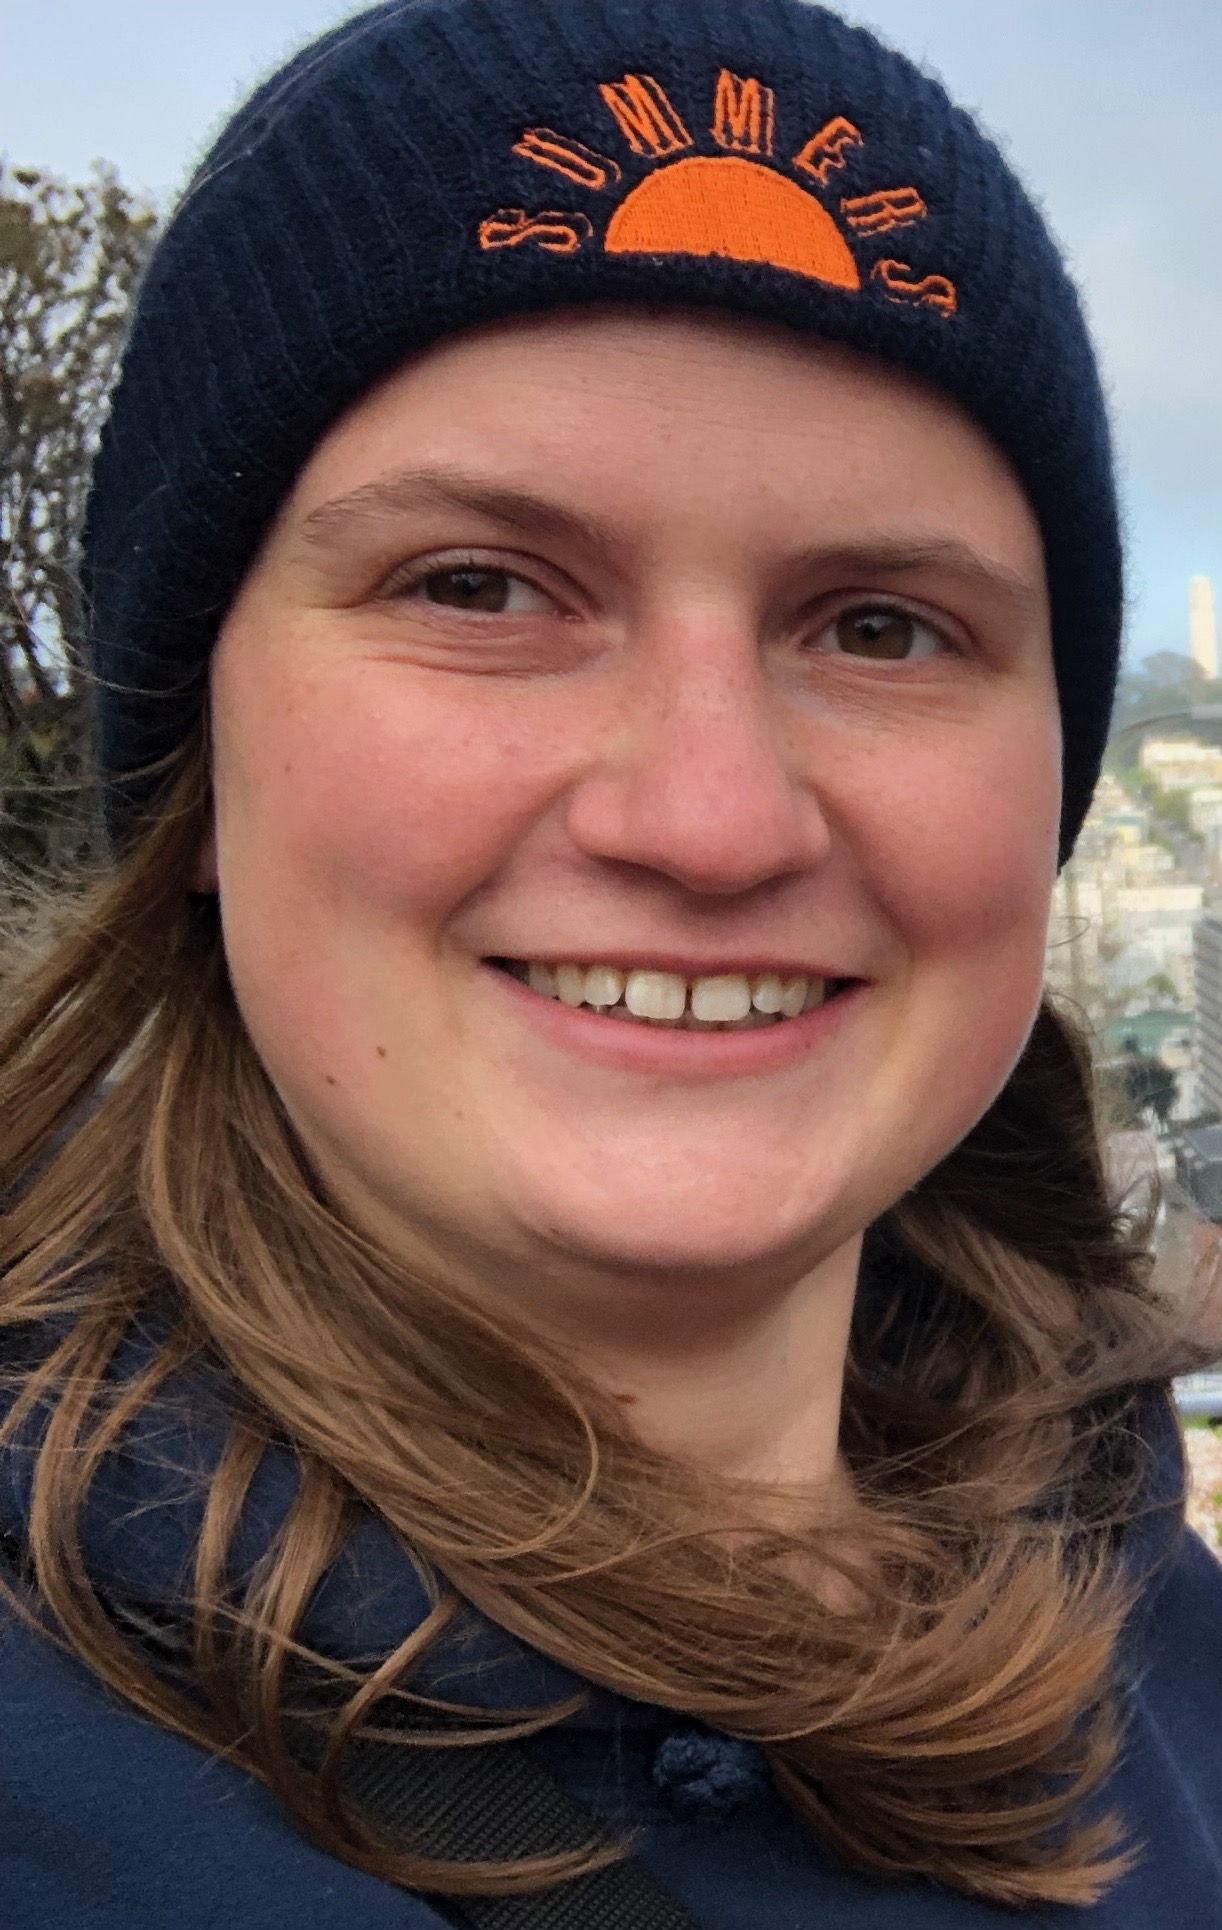
\includegraphics[height=0.35\textheight]{anna.jpeg}
      \end{minipage} \hfill
      \begin{minipage}[c]{.4\textwidth}
        \caption*{Anna Summers \\Uni Kiel}
      \end{minipage}
    \end{figure}
  \end{minipage}
  \hspace{0.1\textwidth}
  \begin{minipage}{.28\textwidth}
    \begin{figure}
      \begin{minipage}[c]{.57\textwidth}
        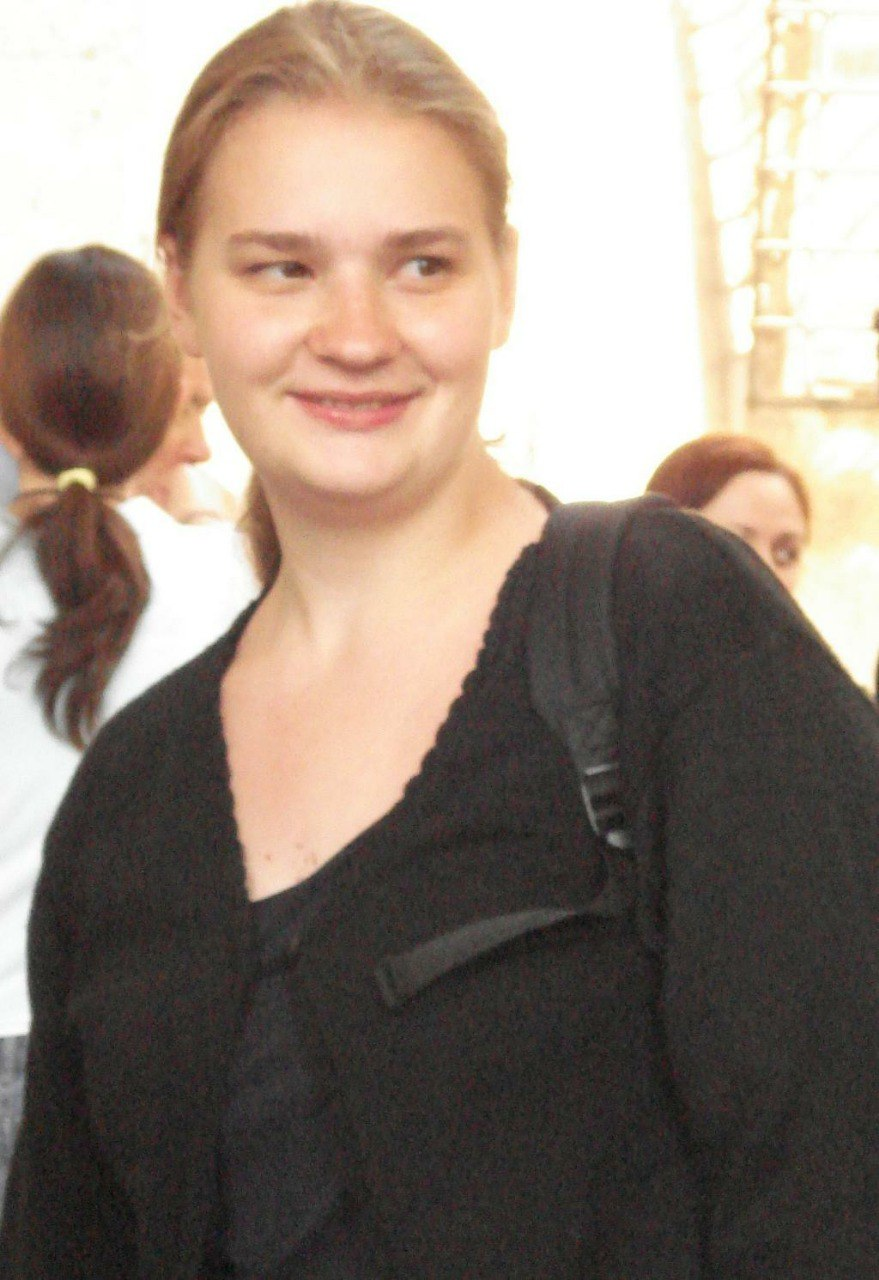
\includegraphics[height=0.35\textheight]{vicky.jpg}
      \end{minipage} \hfill
      \begin{minipage}[c]{.4\textwidth}
        \caption*{Victoria Schemenz \\Alumna}
      \end{minipage}
    \end{figure}
  \end{minipage}
  \hspace{0.1\textwidth}

\end{frame}

\section{Was bisher geschah...}

\begin{frame}{Was bisher geschah...}
  \begin{itemize}
    \item Offener Brief zum Hochchulgesetz NRW versandt und beworben
    \item Resolutionen verschickt und veröffentlicht
    \begin{itemize}
        \item Resolution zu Semesterzeiten \\
          (mit KaWuM, BuFaTa ET, Komet, GeoDACH, BuFaK WiSo, PsyFaKo)
        \item Resolution zu Prüfungsunfähigkeitsbescheinigungen \\
          (mit KaWuM, BuFaTa ET, Komet, GeoDACH, BuFaK WiSo, PsyFaKo, KoPF, KIF)
        \item Resolution zur Wissenschaftskommunikation
        \item Resolution zu Fridays for Future
        \item Resolution zu Lern- und Arbeitsräume
    \end{itemize}
  \end{itemize}
\end{frame}

\begin{frame}{Ganz viele Diskussionen ...}
  \begin{itemize}
    \item Kommunikationswege der ZaPF
    \item Planen neuer Workshops (Gewaltfreie Kommunikation, mentale Gesundheit, ...)
    \item Austausch zu WissKomm ($\rightarrow$ siehe eigener Bericht)
    \item Gespräch mit dem Wissenschaftsrat über studentische Beteiligung an Hochschulen
    \item Kommende Orgas finden \& beraten
    \item Koordinierung von Großprojekten (BaMa-Umfrage, Reformforum, Studienführer, ...)
    \item Viele Kleinigkeiten ...
  \end{itemize}
\end{frame}

\begin{frame}{... und Beschlüsse}
  \begin{itemize}
      \item Mandat für Marcus Mikorski und Jeanette Gehlert zum Thema Wissenschaftskommunikation
      \item Keine Unterstützung der Petition "Menschenrechte für Assange" des FIfF (Forum InformatikerInnen für Frieden und gesellschaftliche Verantwortung)
      \item Mitunterzeichnung des studentischen Forderungskatalogs und \\
      eines offenen Briefs anlässlich der Corona-Krise
      \item Veto im Bündnis Solidarsemester, den Rücktritt von Anja Karliczek zu fordern
      \item Kommende ZaPFen:
        \begin{itemize}
          \item Sommer-ZaPF 2021: Fachschaften Rostock \& Greifswald
          \item Winter-ZaPF 2021/22: Fachschaft Göttingen
        \end{itemize}
    \item Außerplanmäßige Digital-ZaPF
  \end{itemize}
\end{frame}

\begin{frame}
  \begin{itemize}
    \item ZaPF-Bericht verschickt und veröffentlicht
    \item Evaluation aus Freiburg ausgewertet
    \item 10 Sitzungen seit der ZaPF in Freiburg
    \item Klausurtagung vom 6.-8.12.19 in Rostock zur Nachbereitung von Freiburg
    \item Klausurtagung vom 24.-26.04.20 auf Balkonien zur Vorbereitung der Digital ZaPF
    \item Planung der Digital-ZaPF nach der Absage aus Rostock
  \end{itemize}
  \vspace{5mm}
  \begin{center}
    \Large DANKE an alle, die uns dabei unterstützt haben!
  \end{center}
\end{frame}

%\section{Rückmeldungen}

%\begin{frame}{BMBF}
 %   \item Es gab eine Anfrage und zwei Nachfragen an das BMBF
  %   \item Antwort: Nicht genügend Mittel in Förderrunde 2017/2018
   %  \item Prinzipiell steht einer Förderung der nächsten ZaPFen nichts entgegen
 % \end{itemize}
%\end{frame}


\section{Akkreditierung}

\begin{frame}{Akkreditierungspool}
    \begin{itemize}
        \item Der studentische Akkreditierungspool
        \begin{itemize}
        	\item sorgt für die Einflussnahme von Studierenden in Akkreditierungsverfahren
        	\item entsendet Studierendenvertreter in den Akkreditierungsrat und in Agentur- und (extern besetzte) Hochschulgremien
        	\item vertritt studentische Interessen gegenueber Agenturen und anderen Stakeholdern
        \end{itemize}         
        \item Studierende werden vorher in Seminaren geschult. \\
          {\scriptsize\color{blue} N"achste Termine: siehe Webseite \url{https://www.studentischer-pool.de}}
        \item Nächstes Poolvernetzungstreffen wohl digital {\color{blue} (Juni/Juli)}
        \vspace{0.5cm}
        \item[$\rightarrow$] Bei Interesse: Besucht den Akkreditierungs-Workshop f"ur Einsteiger
    \end{itemize}
\end{frame}

%%%%%%%%%%%%%%%%%%%%%%%%%%%%%%%%%%%%%%%%%%%%%%%%%%%%%%%%%%%
% Ab hier nur als Vorlage des StAPF Berichts aus Freiburg %
% Bitte Daten aktualisieren und Informationen anpassen    %
%%%%%%%%%%%%%%%%%%%%%%%%%%%%%%%%%%%%%%%%%%%%%%%%%%%%%%%%%%%

\section{MeTaFa}

 \begin{frame}{MeTaFa}
  \begin{itemize}
    \item Treffen in Erlangen (13. bis 15. September 2019)
    \item Die ZaPF war vertreten durch Merten Dahlkemper und Peter Steinmüller
    \item Darum gings:
    \begin{itemize}
        \item Verabschiedung von gemeinsamen Resolutionen
        \item Studienführer 4all
        \item Umsetzung der DSGVO
    \end{itemize}
    \item Nächstes Treffen: In Dortmund (???)
   \end{itemize}
 \end{frame}

\section{Kommende ZaPFen}
\begin{frame}{Kommende ZaPFen}
  \begin{itemize}
    % \vspace{05cm}
    \item Wintersemester 2020 in München
    \item Sommersemester 2021 in Rostock und Greifswald
    \item Wintersemester 2021 in Göttingen
    \end{itemize}
    \vspace{1cm}
    \begin{center}
      \huge \textbf{Tosenden Applaus für die ausrichtenden Orgas!}
    \end{center}
\end{frame}

\begin{frame}[plain]
  \begin{center}
    \Huge Habt ihr Fragen an uns?
    \end{center}
\end{frame}

\section{KommGrem}

\begin{frame}\frametitle{KomGrem - Wer sind wir?}

  \begin{figure}
     \begin{subfigure}[t]{0.24\textwidth}
       
\includegraphics[height=.5\textheight]{brunner.jpg}
       \caption*{Jacob Brunner (Augsburg)}
     \end{subfigure}
       \begin{subfigure}[t]{0.24\textwidth}
         
\includegraphics[height=.5\textheight]{blaensdorf.jpg}
         \caption*{Sebastian Blänsdorf (Heidelberg)}
     \end{subfigure}
       \begin{subfigure}[t]{0.24\textwidth}
         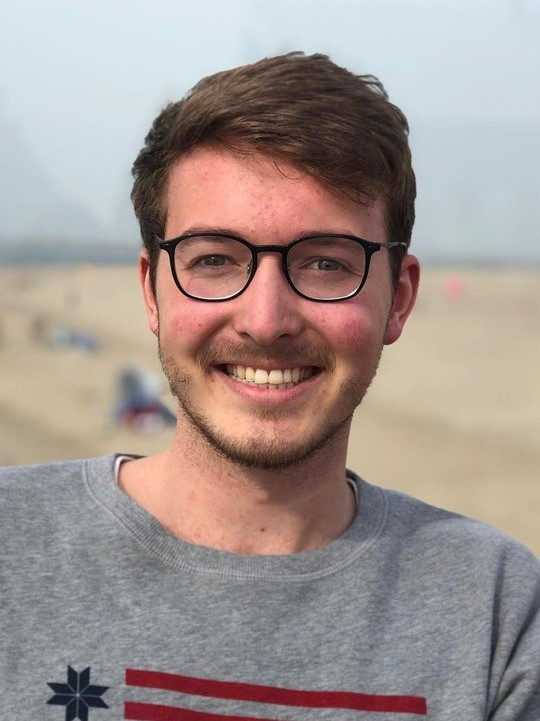
\includegraphics[height=.5\textheight]{Nitschke.jpeg}
         \caption*{Jonah Nitschke (jDPG RG Dortmund)}
     \end{subfigure}
         \begin{subfigure}[t]{0.24\textwidth}
         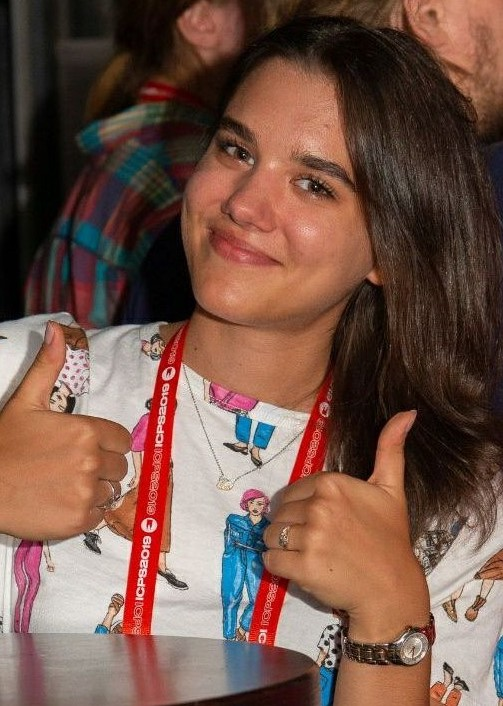
\includegraphics[height=.5\textheight]{boushmelev.jpg}
         \caption*{Anastasia Boushmelev (jDPG RG Siegen)}
     \end{subfigure}
  \end{figure}
 \end{frame}
 
 \begin{frame}\frametitle{KomGrem - Was machen wir?}
 
   \begin{block}{Was wir machen}
     \begin{itemize}
       \item Koordinierung der Zusammenarbeit von jDPG und ZaPF
       \item Austausch über mögliche Kooperationen bei verschiedenen Themen (CHE, Nachhaltigkeit etc.)
       \item Teilnahme an der KFP (Konferenz der Fachbereiche Physik)
       \item Verbesserung der Vernetzung zwischen Fachschaften und jDPG Regionalgruppen
     \end{itemize}
   \end{block}
 \end{frame}

%\section{ZaPF e.V.}

\begin{frame}{Was tut der ZaPF e.V.?}
  \begin{block}{Aufgaben des e.V.}
    \begin{itemize}
      \item Strukturelle Unterstützung der ZaPF
      \item Infrastruktur
      \item Finanzielle Absicherung
      \item Rechtliche Absicherung
      \item Finanzierung für Gremien (z.B. Reisekosten)
      \item Unterstützung von Finanzschwachen Fachschaften
    \end{itemize}
  \end{block}
\end{frame}
  
\begin{frame}{Wer tut da was im ZaPF e.V.?}
  \begin{block}{Aktuelle Vorstände}
    \begin{minipage}{0.5\textwidth}
      \begin{figure}
      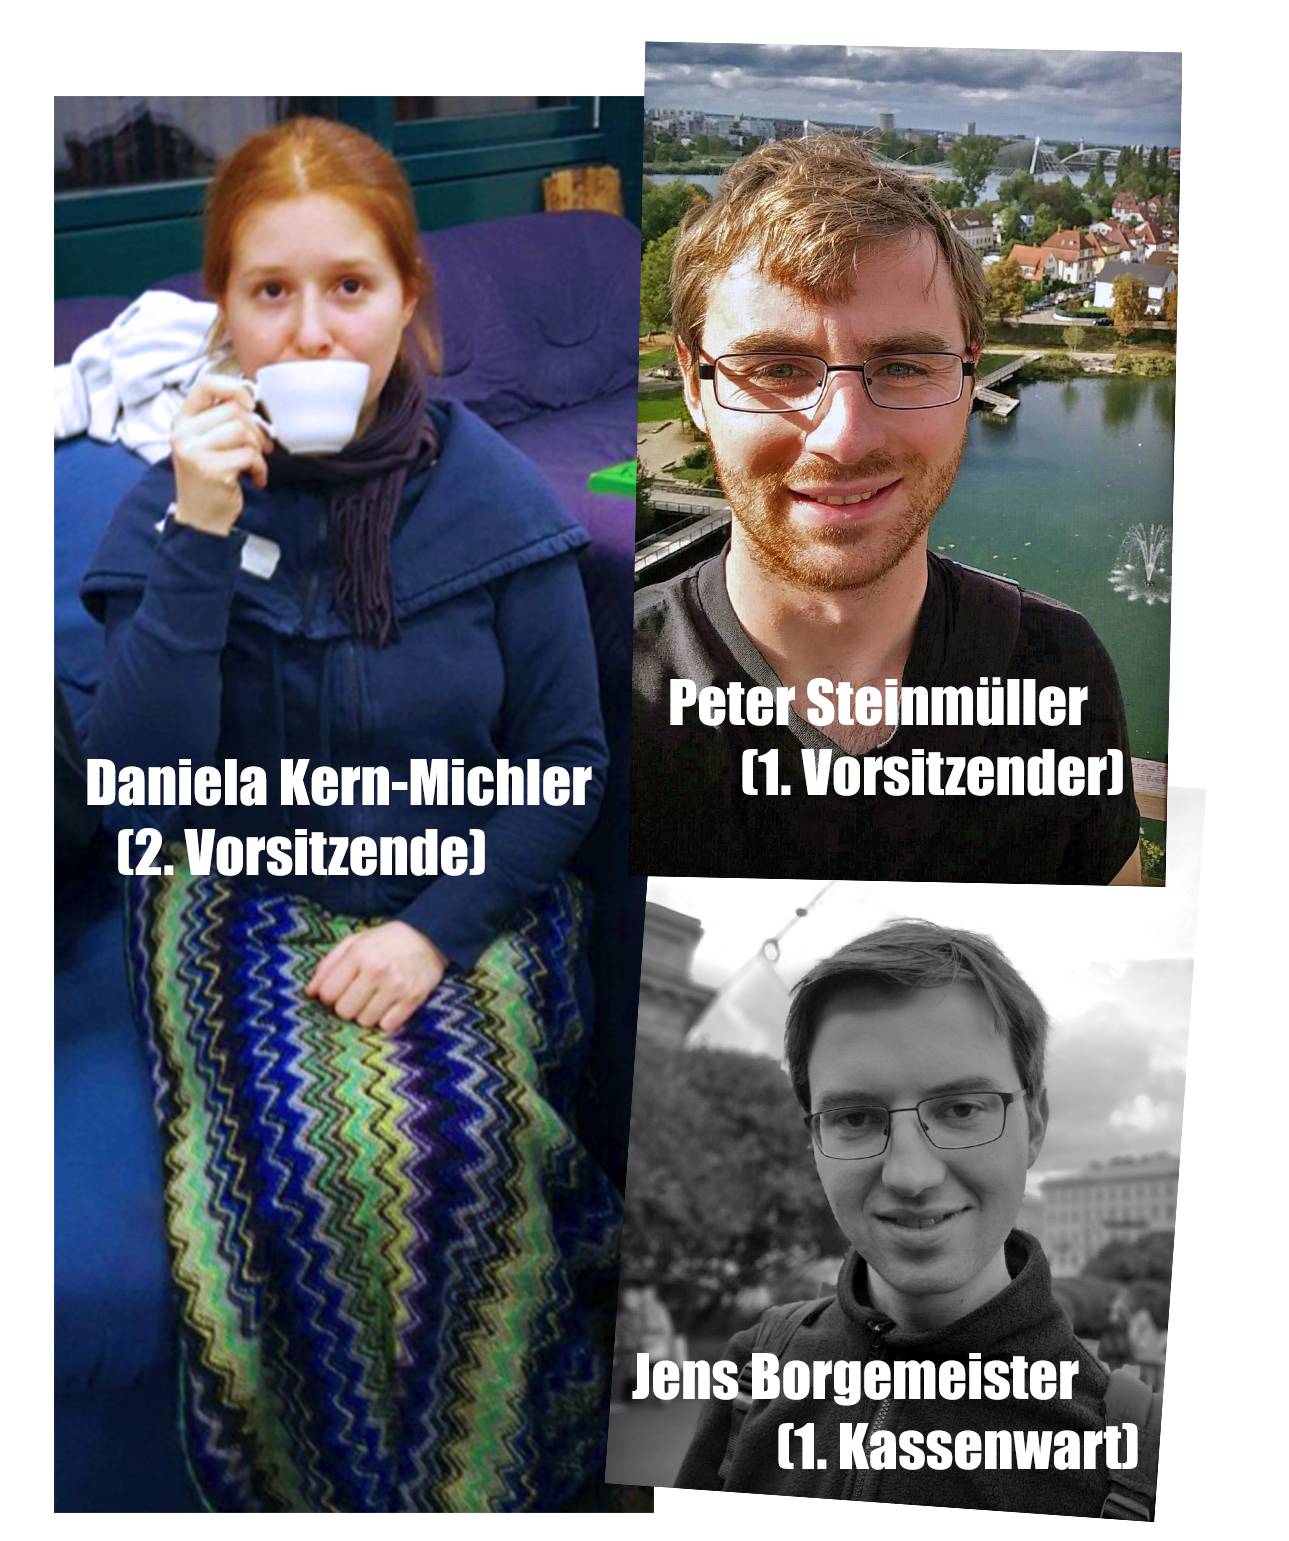
\includegraphics[height=.75\textheight]{ZapfeV.png}
      \end{figure}
    \end{minipage}
    \begin{minipage}{0.45\textwidth}
      \begin{itemize}
        \item Marcus Mikorski \mbox{(2. Kassenwart)}
        \item Fabian Freyer (IT)
        \item Lisa Dietrich (Finanzschwache Fachschaften)
        \item Marcel Nitsch (Bonn)
        \item Timo Rachel (Freiburg)
        \item Lena Wunderl (München)
        \item Richard Altenkirch (Rostock)
      \end{itemize}
    \end{minipage}
  \end{block}
\end{frame}
  
\begin{frame}{Was kann man tun im ZaPF e.V.?}
  \begin{block}{Fördermitglied werden}
    Fachschaften unterstützen den e.V. mit Mitgliedsbeiträgen
  \end{block}
  \begin{block}{Mitglied werden}
    Kommt zur Mitgliederversammlung!
  \end{block}
\end{frame}
  
\begin{frame}{Mitgliederversammlung am 6.6. um 14 Uhr}
  \begin{block}{Tagesordnung}
    \begin{multicols}{2}
      \begin{enumerate}\small
        \item Feststellung der Tagesordnung
        \item Wahl des Protokollführers
        \item Wahl der Versammlungsleitung
        \item Feststellung der Beschlussfähigkeit
        \item Genehmigung der letzten Protokolle
        \item Bericht des Vorstands
        \item Bericht des Kassenprüfers
        \item Mitgliedschaft und Versicherung beim Deutschen Ehrenamt e.V.
        \item Datenschutz
        \item Reisekostenerstattung
        \item Änderung des Postens "Finanzschwache Fachschaften"
        \item Sonstiges
      \end{enumerate}
    \end{multicols}
  \end{block}
\end{frame}

\begin{frame}{Was ist der TOPF?}
  \begin{minipage}{.5\textwidth}
    \begin{itemize}
      \item 2 DECkEL \footnotemark[1]
      \begin{itemize}
        \item Sean Bonkwoski (Bonn)
        \item Timo Prinz (Berlin, TU)
      \end{itemize}
      \item Viele HENkeL\footnotemark[2]\footnotemark[3]
      \item Server
      \item ... und ganz viele Dienste
    \end{itemize}
  \end{minipage}
  \hfill
  \begin{minipage}{.48\textwidth}
    \begin{minipage}[c]{.5\textwidth}
      
\includegraphics[height=.4\textheight]{dummy.jpg}
      \captionof*{figure}{Sean}
    \end{minipage}
    \begin{minipage}[c]{.48\textwidth}
      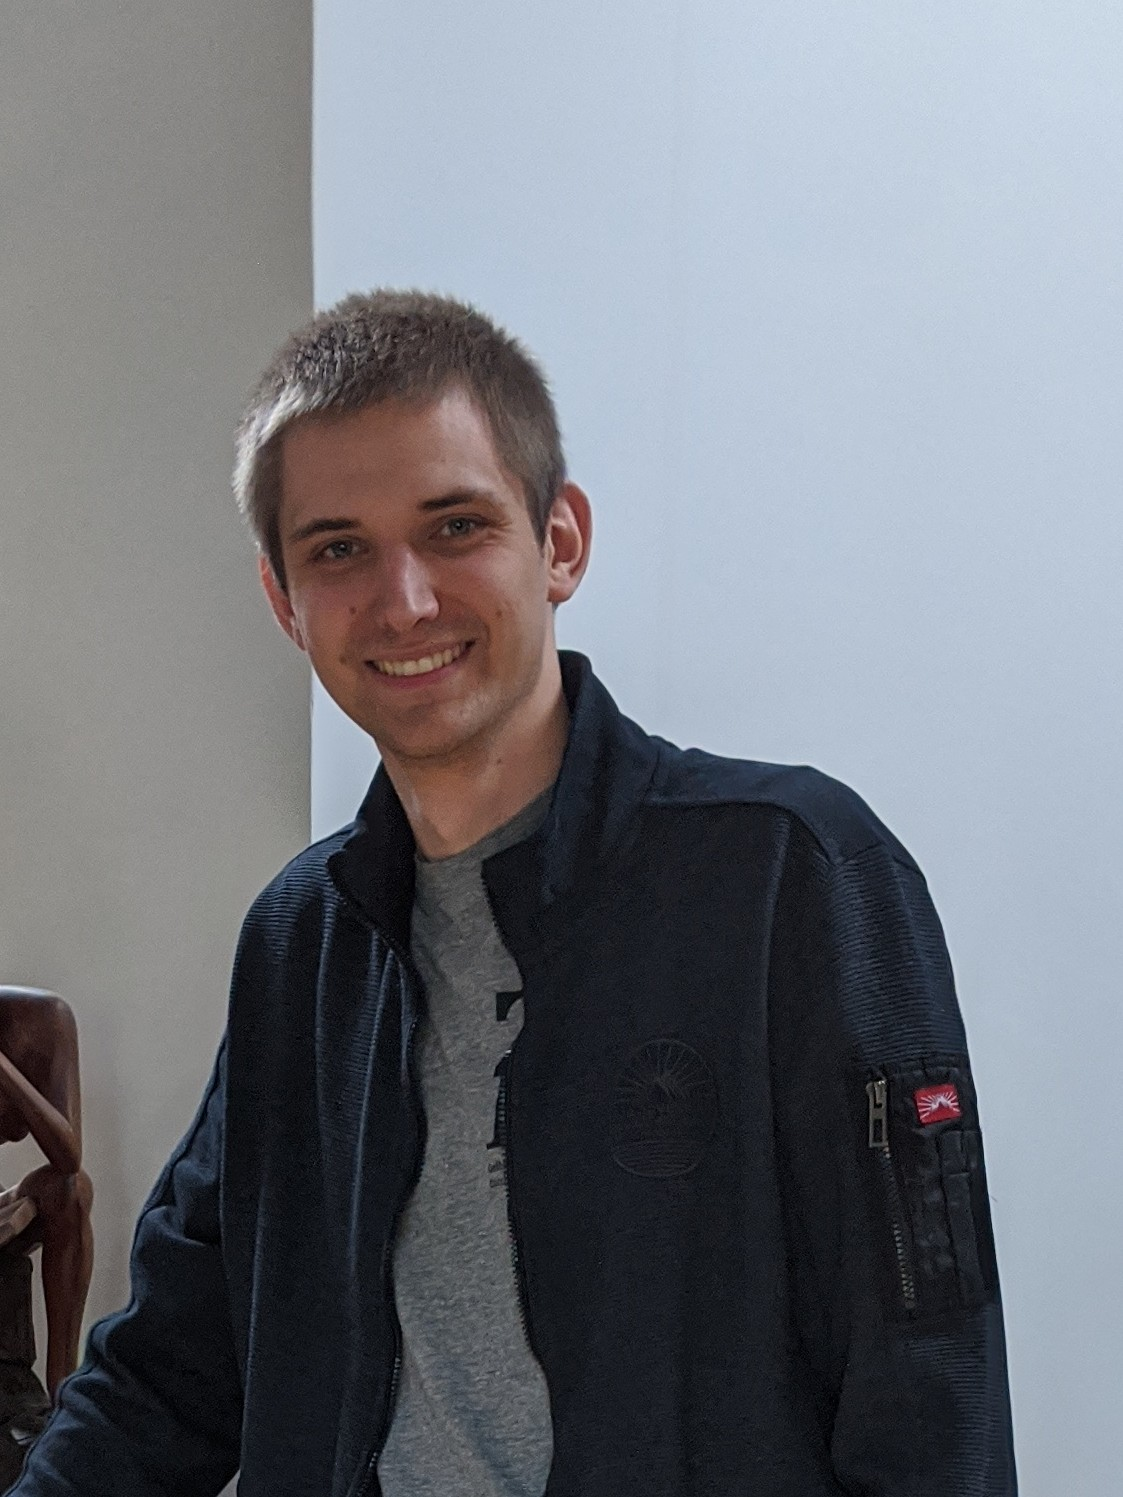
\includegraphics[height=.4\textheight]{timo.jpg}
      \captionof*{figure}{Timo}
    \end{minipage}
  \end{minipage}
  \footnotetext[1]{Dokumentations-, Einrichtungs- und Clusterfuckkoordinierende für EDV-Lösungen} 
  \footnotetext[2]{Helfende mit EDV- und Netzwerkkompetenzen für ergebnisorentierte Lösungen}
  \footnotetext[3]{Können gerne mehr werden ;-)}
\end{frame}

% \pagestyle{empty}
% \begin{frame}{Was tut der TOPF?}
% \begin{block}{Aufgaben der DECkEL:}
% \begin{itemize}
% \item Vorhandene Dienste am laufen und aktuell halten
% \item Gremika Rechte geben und entziehen
% \item Dienste für Orgas der nächsten ZaPFen bereitstellen
% \item HENkeL koordiniern
% \end{itemize}
% \end{block}
% \pause
% \begin{block}{Aufgaben der HENkeL}
%   \begin{itemize}
%     \item Entwicklung und Einrichtung neuer Dienste
%     \item Generell Hilfe und Entlastung der DECkEL
%   \end{itemize}
% \end{block}
% \end{frame}

% \pagestyle{empty}
% \begin{frame}{Was hat der TOPF seit Bonn getan?}
%   \begin{itemize}
%     \item WOLKe\footnote{Wissens-Online-Lager für Kompetenzerhaltung} eingerichtet (Nur für Gremienarbeit)
%     \item ZapF-Wiki-Anmeldung jetzt über ZaPF-Account
%     \item Datenschutz-Überarbeitung mit ZaPF-e.V.-Vorstand
%     \item Dinge für ZaPF in Freiburg (Anmeldung, App, ...)
%   \end{itemize}
% \end{frame}

% \pagestyle{empty}
% \begin{frame}{Was hat der TOPF noch zu tun?}
%   Arbeit geht uns nie aus.
%   \begin{itemize}
%     \item Alten Server abschalten (fast fertig!)
%     \item Backups!
%     \item Datenschutz-Überarbeitung fortsetzen
%     \item Dinge für Ostsee-ZaPF (Anmeldung, App, ...)
%     \item und vieles mehr
%   \end{itemize}
% \end{frame}

\end{document}
